\documentclass[12pt,a4paper]{article}
\usepackage[utf8]{vietnam}
\usepackage{amsmath,amssymb}
\usepackage{tabularx}
\usepackage{tikz}
\usetikzlibrary{calc,angles,quotes,arrows.meta,patterns}
\usepackage{xcolor}
\usepackage{enumitem}
\usepackage{fancyhdr}
\usepackage{graphicx}
\usepackage[top=0.9cm, bottom=0.9cm, left=1.2cm, right=1.2cm]{geometry}
\usepackage[dethi]{ex_test}
\SAOPTN{widthSA=3.2,heightSA=0.62}

\setlength{\headheight}{15pt}
\setlength{\parskip}{0pt}

\pagestyle{fancy}
\fancyhf{}
\rhead{\textit{Môn Toán 9 -- Đề số 03}}
\lhead{\textit{Bộ đề ôn tập Giữa học kì I}}
\cfoot{\thepage}

\begin{document}

% --- KHUNG TIÊU ĐỀ ĐỀ THI ---
\noindent
\begin{tabularx}{\linewidth}{X r}
\textbf{TRƯỜNG THCS: \dotfill} & \textbf{ĐỀ KIỂM TRA ĐỊNH KỲ GIỮA HỌC KỲ I} \\
\textbf{Họ và tên: \dotfill} & \textbf{NĂM HỌC 2026 -- 2027} \\
\textbf{Lớp: \dotfill \quad SBD: \dotfill} & \textbf{Môn: TOÁN 9} \\
\hline
\end{tabularx}
\vspace{2mm}

\begin{center}
  \textbf{\large ĐỀ ÔN TẬP GIỮA HỌC KỲ I -- ĐỀ SỐ 03}\\
  \textit{Thời gian làm bài: 90 phút (Không kể thời gian phát đề)}
\end{center}
\vspace{1mm}

% --- PHẦN I ---
\noindent\textbf{\large PHẦN I. CÂU TRẮC NGHIỆM NHIỀU PHƯƠNG ÁN LỰA CHỌN (3,0 điểm)}

\textit{Thí sinh trả lời từ câu 1 đến câu 12. Mỗi câu hỏi thí sinh chỉ chọn một phương án duy nhất.}

\vspace{1mm}
\begin{ex}
Phương trình nào sau đây là phương trình bậc nhất hai ẩn?
\choice
{$2x^2 - 3y = 1$}
{\True $x - 3y = 1$}
{$3x^2 + 2y = 1$}
{$0x + 0y = 1$}
\end{ex}

\begin{ex}
Phương trình nào dưới đây nhận cặp số $(-2; 4)$ làm nghiệm?
\choice
{\True $2x + y = 0$}
{$x - y = 1$}
{$x - 2y = 0$}
{$x + 2y + 1 = 0$}
\end{ex}

\begin{ex}
Phương trình $(x^2 + 9)(2x + 3) = 0$ có số nghiệm là:
\choice
{$0$}
{\True $1$}
{$2$}
{$3$}
\end{ex}

\begin{ex}
Hệ phương trình nào sau đây có vô số nghiệm?
\choice
{$\begin{cases} 2x - 5y = 1 \\ -x + 3y = 2 \end{cases}$}
{$\begin{cases} 2x - 5y = 1 \\ x + 3y = 2 \end{cases}$}
{\True $\begin{cases} 2x - 5y = 1 \\ -x + \frac{5}{2}y = -\frac{1}{2} \end{cases}$}
{$\begin{cases} 2x - 5y = 1 \\ -x - 3y = 2 \end{cases}$}
\end{ex}

\begin{ex}
Nghiệm của hệ phương trình $\begin{cases} 4x = 8 \\ 3x + 2y = 10 \end{cases}$ là:
\choice
{$(1; 2)$}
{$(2; 3)$}
{$(3; 4)$}
{\True $(2; 2)$}
\end{ex}

\begin{ex}
Cho hệ phương trình $\begin{cases} 4x - y = 2 \\ x + 3y = 7. \end{cases}$ Cặp số nào dưới đây là nghiệm của hệ phương trình đã cho?
\choice
{$(2; 2)$}
{\True $(1; 2)$}
{$(-1; -2)$}
{$(2; -2)$}
\end{ex}

\begin{ex}
Trong các cặp số sau, cặp số nào là nghiệm của phương trình $x + y = 3$?
\choice
{$(8; 1)$}
{$(-3; 6)$}
{\True $(4; -1)$}
{$(0; 2)$}
\end{ex}

\begin{ex}
Cặp số $(x; y) = (3; -1)$ là nghiệm của hệ phương trình nào sau đây?
\choice
{\True $\begin{cases} 2x + y = 5 \\ 3x - 2y = 11 \end{cases}$}
{$\begin{cases} 2x + 2y = 5 \\ 3x - 2y = 11 \end{cases}$}
{$\begin{cases} 2x + y = 6 \\ 3x - 2y = 1 \end{cases}$}
{$\begin{cases} 2x + y = -6 \\ 3x + y = 10 \end{cases}$}
\end{ex}

\begin{ex}
Cho tam giác $ABC$ vuông tại $A$. Khi đó tỉ số lượng giác $\tan B$ bằng:
\choice
{$\frac{AB}{BC}$}
{$\frac{AC}{BC}$}
{$\frac{CB}{BA}$}
{\True $\frac{AC}{AB}$}
\end{ex}

\begin{ex}
Cho tam giác $ABC$ vuông tại $A$, đường cao $AH \perp BC$ ($H \in BC$). Biết $AH = 6, BH = 3$. Giá trị $\sin B$ bằng:
\choice
{$\frac{\sqrt{3}}{3}$}
{$\frac{\sqrt{3}}{2}$}
{\True $\frac{2\sqrt{5}}{5}$}
{$\frac{\sqrt{3}}{6}$}
\end{ex}

\begin{ex}
Cho tam giác $ABC$ vuông tại $A$, đường cao $AH \perp BC$ ($H \in BC$). Biết $BH = 3, HC = 1$. Số đo góc $B$ là:
\choice
{\True $30^\circ$}
{$60^\circ$}
{$70^\circ$}
{$45^\circ$}
\end{ex}

\begin{ex}
Cho hình vẽ tam giác vuông $ABH$ vuông tại $H$ với $BH = 10\text{ m}$ và $\widehat{B} = 60^\circ$. Chiều cao $AH$ có độ dài là:
\begin{center}
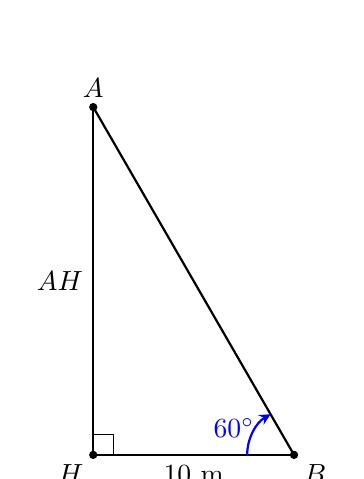
\begin{tikzpicture}[scale=0.85, line join=round, line cap=round, >=stealth]
  \coordinate (H) at (0,0);
  \coordinate (B) at (3,0);
  \coordinate (A) at (0,5.196); % 3 * sqrt(3)
  \draw[thick] (H) -- (B) node[midway, below] {$10\text{ m}$};
  \draw[thick] (A) -- (H) node[midway, left] {$AH$};
  \draw[thick] (A) -- (B);
  \draw (0,0.3) -- (0.3,0.3) -- (0.3,0);
  \draw[->, thick, blue] (2.3,0) arc (180:120:0.7);
  \node at (2.1,0.4) [blue] {$60^\circ$};
  \filldraw[black] (H) circle (1.5pt) node[below left] {$H$};
  \filldraw[black] (B) circle (1.5pt) node[below right] {$B$};
  \filldraw[black] (A) circle (1.5pt) node[above] {$A$};
\end{tikzpicture}
\end{center}
\choice
{$20\text{ m}$}
{\True $10\sqrt{3}\text{ m}$}
{$15\sqrt{3}\text{ m}$}
{$20\sqrt{3}\text{ m}$}
\end{ex}


\vspace{1mm}
\noindent\textbf{BẢNG TRẢ LỜI TRẮC NGHIỆM PHẦN I:}
\begin{center}
\begin{tabular}{|c|c|c|c|c|c|c|c|c|c|c|c|c|}
\hline
\textbf{Câu} & \textbf{1} & \textbf{2} & \textbf{3} & \textbf{4} & \textbf{5} & \textbf{6} & \textbf{7} & \textbf{8} & \textbf{9} & \textbf{10} & \textbf{11} & \textbf{12} \\
\hline
\textbf{Chọn} & \rule{0pt}{0.65cm} & & & & & & & & & & & \\
\hline
\end{tabular}
\end{center}
\vspace{2mm}

\setcounter{ex}{0}
\noindent\textbf{\large PHẦN II. CÂU TRẮC NGHIỆM ĐÚNG SAI (2,0 điểm)}

\textit{Thí sinh trả lời câu 1 và câu 2. Trong mỗi ý a), b), c), d) ở mỗi câu, thí sinh chọn đúng hoặc sai.}

\vspace{1mm}
\begin{ex}
Cho hệ phương trình $\begin{cases} 6x - y = -12 \quad (1) \\ 2x + y = 4 \quad (2). \end{cases}$ Xét tính Đúng/Sai của các khẳng định sau:
\choiceTF
{\True Hệ phương trình trên là hệ hai phương trình bậc nhất hai ẩn}
{Hệ phương trình trên là hệ phương trình bậc nhất một ẩn}
{Cộng phương trình (1) và (2) vế theo vế, ta được phương trình $8x = 16$}
{\True Nghiệm của hệ phương trình trên là $(-1; 6)$}
\end{ex}

\begin{ex}
Cho tam giác $ABC$ vuông tại $A$, biết $AB = 4\text{ cm}$ và $AC = 3\text{ cm}$. Xét tính Đúng/Sai của các khẳng định sau:
\choiceTF
{\True $\tan B = \frac{AC}{AB} = \frac{3}{4}$}
{\True Số đo góc $\widehat{B} \approx 37^\circ$}
{Cạnh huyền $BC = AC \cdot \sin B$}
{\True $\tan C = \cot B = \frac{4}{3}$}
\end{ex}


\noindent\textbf{BẢNG TRẢ LỜI PHẦN II:}
\begin{center}
\begin{tabular}{|c|c|c|c|c||c|c|c|c|c|}
\hline
\textbf{Câu 1} & \textbf{a)} & \textbf{b)} & \textbf{c)} & \textbf{d)} & \textbf{Câu 2} & \textbf{a)} & \textbf{b)} & \textbf{c)} & \textbf{d)} \\
\hline
\textbf{Đ/S} & \rule{0pt}{0.6cm} & & & & \textbf{Đ/S} & & & & \\
\hline
\end{tabular}
\end{center}
\vspace{2mm}

\setcounter{ex}{0}
\noindent\textbf{\large PHẦN III. CÂU HỎI TRẢ LỜI NGẮN (2,0 điểm)}

\textit{Thí sinh trả lời câu 1 và câu 2. Điền kết quả vào ô trống tương ứng.}

\vspace{1mm}
\begin{ex}
Tổng số học sinh nam và nữ trong một lớp là $40$. Số học sinh nam nhiều hơn số học sinh nữ là $4$ bạn. Hỏi lớp có bao nhiêu học sinh nam và bao nhiêu học sinh nữ? \shortans{Nam: 22, Nữ: 18}
\end{ex}

\begin{ex}
Cho đường tròn $(O)$ có số đo cung $\text{sđ}\, \wideparen{AmB} = 62^\circ$. Số đo góc ở tâm $\widehat{AOB}$ bằng bao nhiêu độ? \shortans{$62^\circ$}
\end{ex}


\setcounter{ex}{0}
\noindent\textbf{\large PHẦN IV. TỰ LUẬN (3,0 điểm)}

\textit{Thí sinh trình bày chi tiết lời giải vào giấy làm bài.}

\vspace{1mm}
\begin{ex} (1,0 điểm)
Giải hệ phương trình và bất phương trình sau:
\begin{enumerate}[label=\textbf{\alph*)}, leftmargin=0.8cm, itemsep=2pt]
\item (0,5 điểm) $\begin{cases} 3x - 2y = 7 \\ x + 4y = 7 \end{cases}$
\item (0,5 điểm) $\frac{x}{3} - \frac{2x - 1}{2} < 1$
\end{enumerate}
\end{ex}
\vspace{0.5mm}

\begin{ex} (0,75 điểm)
Thực hiện các yêu cầu sau:
\begin{enumerate}[label=\textbf{\alph*)}, leftmargin=0.8cm, itemsep=2pt]
\item (0,35 điểm) Dùng kí hiệu toán học để viết bất đẳng thức: Tốc độ của xe gắn máy trên đoạn đường này phải đạt tối thiểu $40\text{ km/h}$.
\item (0,4 điểm) Cho $a > b$, chứng minh rằng: $2 - 5a < 2 - 5b$.
\end{enumerate}
\end{ex}
\vspace{0.5mm}

\begin{ex} (0,75 điểm)
Hai trạm quan trắc tàu biển đặt ở hai mỏm núi $A$ và $B$ cách nhau $2\text{ km}$, nhìn thấy chiếc tàu $C$ ở phía xa với góc $\widehat{CAB} = 50^\circ$ và $\widehat{CBA} = 45^\circ$. Hỏi tàu $C$ còn cách đường thẳng $AB$ bao nhiêu mét?
\begin{center}
\begin{tikzpicture}[scale=1.1, line join=round, line cap=round, >=stealth]
  \coordinate (A) at (0,0);
  \coordinate (B) at (4,0);
  \coordinate (H) at (1.8,0);
  \coordinate (C) at (1.8,2.2);
  \draw[thick] (-0.5,0) -- (4.5,0) node[below] {Bờ biển $(AB)$};
  \draw[thick, blue] (A) -- (C) -- (B);
  \draw[thick, dashed, red] (C) -- (H) node[midway, left] {$h$};
  \draw (1.8,0.2) -- (2.0,0.2) -- (2.0,0);
  \draw[->, thick, purple] (0.7,0) arc (0:50:0.7);
  \node at (1.0,0.3) [purple] {$50^\circ$};
  \draw[->, thick, purple] (3.3,0) arc (180:135:0.7);
  \node at (3.0,0.3) [purple] {$45^\circ$};
  \filldraw[black] (A) circle (1.5pt) node[below left] {$A$};
  \filldraw[black] (B) circle (1.5pt) node[below right] {$B$};
  \filldraw[black] (H) circle (1.5pt) node[below] {$H$};
  \filldraw[black] (C) circle (1.5pt) node[above] {Tàu $(C)$};
  \node at (2,-0.4) {$AB = 2000\text{ m}$};
\end{tikzpicture}
\end{center}
\end{ex}
\vspace{0.5mm}

\begin{ex} (0,5 điểm)
Hai ô tô cùng khởi hành một lúc từ $A$ đến $B$ cách nhau $150\text{ km}$. Biết vận tốc ô tô thứ nhất lớn hơn vận tốc ô tô thứ hai là $10\text{ km/h}$ và ô tô thứ nhất đến $B$ trước ô tô thứ hai là $30\text{ phút}$. Tính vận tốc của mỗi ô tô.
\end{ex}
\vspace{0.5mm}


\enlargethispage{1.5cm}
\begin{center}
\rule{4cm}{0.4pt}\\
\textit{--- HẾT ---}
\end{center}
\end{document}
